\chapter{Analysing C++ code}
\label{chap:AnalysingCPP}

To retrieve information about elements declared in C++ header files a shared library called \textbf{CPPAnalyzer} was written in C++. The library uses \textbf{libclang} for parsing C++ files and accessing AST information. Internally a reduced syntax tree is built and exported as JSON (JavaScript Object Notation).\todo{explain json}

The library exposes its functionality in form of a C interface. It uses features from the new C++ standard C++11 (including the ''auto'' keyword, but more importantly the regular expression functionality of the standard library). CPPAnalyzer is currently build using Visual Studio 2010 on Windows 7 64-bit. Other operating systems or compilers have not been tested, but should be supported with minor modifications.

\section{libclang}

As explained in \myRefSection{sec:Clang}, libclang is a C interface to Clang that can be used for accessing Clang's parsing functionality and internal AST.

\todo{explain AST stuff}

The two most important data structures libclang provides, are CXCursor and CXType.
\\\textbf{CXCursor} represents a single node in the AST. It holds an enum constant (named kind) that identifies the kind of the AST node - whether it is a namespace, function declaration, class declaration, etc. It also saves information about the according Clang data in an array of void pointers.
\\\textbf{CXType} represents a C++ type. It holds the kind of the type, for example if it is a pointer, reference, builtin type (like int or float), record (class or struct), etc. Just like CXCursor, it also saves information about the Clang type representation.

More information about cursors and types can be retrieved using the functions libclang provides.
\\If the user, for example, wants to know if a member function is declared as ''virtual'', he will call \mySCName{clang\_isCXXMethodVirtual} and pass a cursor that represents a member function (e.g. with the kind \mySCName{CXCursor\_CXXMethod}) to it. \mySCName{clang\_getCursorType}, as another example, will return the type of a variable or parameter declaration as a CXType.

\mySCName{clang\_parseTranslationUnit} is the starting point for parsing C++ files. The function ''accepts a set of command-line arguments so that the compilation can be configured in the same way that the compiler is configured on the command line''\todo{ref}. These options commonly contain the path to the file to be parsed. The function returns a translation unit, which holds all the AST information and is also the root cursor of the AST. While parsing, Clang produces diagnostic information, for example when mal-formed C++ code was provided or other errors occur. libclang provides functionality to access these diagnostics.

To traverse the abstract syntax tree (recursively), \mySCName{clang\_visitChildren} is used. As arguments, it takes the cursor to be visited, a function pointer, which serves as a callback that is called for every child, and a void pointer for user data. The callback function will be called from Clang, passing the visited cursor, its parent and the user data as parameters. The callback function is normally used to inspect and analyse the given cursor. The return value of the function tells Clang, if it should go on recursively with the first child of the cursor, go on with the next sibling or if it should end traversing of the AST at this point.

libclang provides more than 50 functions that deal with AST inspection - far too much, to be covered in this thesis. A complete overview is given at the libclang doxygen documentation.\footnote{\url{http://clang.llvm.org/doxygen/group\_\_CINDEX.html}}

\subsection{Extending libclang}

libclang does not expose all of the functionality Clang provides. Functionality missing in libclang is added on a per-need basis. 

During this thesis it became clear that libclang needed to be extended by the author to expose AST information about C++ templates. It seems, such information was not needed by other libclang users. The changes made to the libclang source code base will hopefully make its way back into the official Clang repository.

Most of the functions added to libclang simply forward Clang's internals. Still, the Clang code base needed to be understood and used in a safe\todo{word} fashion.

When turning Clang types into CXTypes, certain C++ types were not exposed. libclang was altered to support template type parameter types (TemplateTypeParm), template specialization types and elaborated types (types that are sugared with a type keyword like ''class'' and/or a prefixed namespace identifier):

\SingleSpacing
\begin{lstlisting}[language=C++, caption=Examples of types now supported by libclang]
template<class T>
class TemplatedClass
{
	// NEW: type of kind TemplateTypeParm
	T member; 
};

// NEW: type of kind TemplateSpecialization
TemplatedClass<int> tempSpecInstance; 

namespace SomeNamespace
{	
	class NormalClass{};
	
	// OLD: type of kind Record
	NormalClass instance;
	
	// NEW: type of kind Elaborated
	class NormalClass elaboratedInstance1;
}

// NEW: type of kind Elaborated
SomeNamespace::NormalClass elaboratedInstance2; 
\end{lstlisting}
\OnehalfSpacing

libclang already exposed template parameters as CXCursors when visiting the children of a class, struct or function cursor. Helper functions for accessing the template parameters directly from a template-supporting cursor, were added to libclang:

\begin{itemize}\addtolength{\itemsep}{-0.5\baselineskip}
\item unsigned clang\_getTemplateNumParameters(CXCursor C);
\item CXCursor clang\_getTemplateParameter(CXCursor C, unsigned Index);
\end{itemize}

libclang did not expose any information about template arguments. Template arguments are the actual types used for template parameters, when instantiating a template. Functions for retrieving template arguments and their values (as type, integral, etc.) were added:

\begin{itemize}\addtolength{\itemsep}{-0.5\baselineskip}
\item Added cursor kinds\begin{itemize}\addtolength{\itemsep}{-0.5\baselineskip}
	\item CXCursor\_TemplateNullArgument
	\item CXCursor\_TemplateTypeArgument
	\item CXCursor\_TemplateDeclarationArgument
	\item CXCursor\_TemplateIntegralArgument
	\item CXCursor\_TemplateTemplateArgument
	\item CXCursor\_TemplateTemplateExpansionArgument
	\item CXCursor\_TemplateExpressionArgument
	\item CXCursor\_TemplatePackArgument
	\end{itemize}
\item Added functions\begin{itemize}\addtolength{\itemsep}{-0.5\baselineskip}
	\item unsigned clang\_isTemplateArgument(CXCursor C);
	\item unsigned clang\_getTemplateSpecializationNumArguments(CXCursor C);
	\item CXCursor clang\_getTemplateSpecializationArgument(CXCursor C, unsigned Index);
	\item CXType clang\_getTemplateArgumentValueAsType(CXCursor C);
	\item long long clang\_getTemplateArgumentValueAsIntegral(CXCursor C);
	\item CXCursor clang\_getTemplateArgumentValueAsDeclaration(CXCursor C);
	\item CXCursor clang\_getTemplateArgumentValueAsTemplate(CXCursor C);
	\item CXCursor clang\_getTemplateArgumentValueAsExpression(CXCursor C);
	\end{itemize}
\end{itemize}

Also a utility function for retrieving the access (private, protected or public) of a C++ member field/function/subclass was added:
\begin{itemize}\addtolength{\itemsep}{-0.5\baselineskip}
\item CX\_CXXAccessSpecifier clang\_getCXXMemberAccessSpecifier(CXCursor)
\end{itemize}

Before, access needed to be tracked while analysing a class/struct cursor's children, by finding special child cursors that represent the C++ access specifiers.

\section{Building a simplified AST}

libclang provides an AST that contains a lot of information, which is not needed for language binding purposes. Thus, a simplified abstract syntax tree is created that holds all necessary information in form of a tree structure.

The creation of the simplified AST is processed inside the \mySCName{Clang\_AST} class and happens roughly in the following steps:

\begin{enumerate}\addtolength{\itemsep}{-0.5\baselineskip}
\item Create an intermediate AST that closely resembles the cursor tree that Clang generates, filtering based on the cursor kind
\item Filter the intermediate tree based on user-given filters for file- and symbol name
\item For the nodes that are left, create data structures (of type \mySCName{ASTObject}) that hold information about the AST node and retrieve its properties using the libclang API. Create data structures that hold type information (\mySCName{ASTType}) along the way.
\item Connect the \mySCName{ASTObject}s to form the final simplified AST 
\end{enumerate}

\subsection{The intermediate AST}

In C++, the same object (a function or class) can be declared multiple times, but only defined once. This property is sometimes used to eliminate unnecessary includes or avoid cyclic file dependencies, by providing forward declarations.\\
In Clang, every declaration is a single AST node. This information is mostly unnecessary for glue code generation, thus AST nodes that represent the same C++ entity are combined in the intermediate AST. libclang provides this functionality with the concept of a \textbf{canonical cursor} - a single cursor that represents the underlying entity.

The intermediate tree is build using instances of \mySCName{Clang\_AST\_CXTreeNode}, which can be seen in \myRefFigure{fig:CXTreeNode}. 

\begin{figure}[h] % h = here
	\centering
		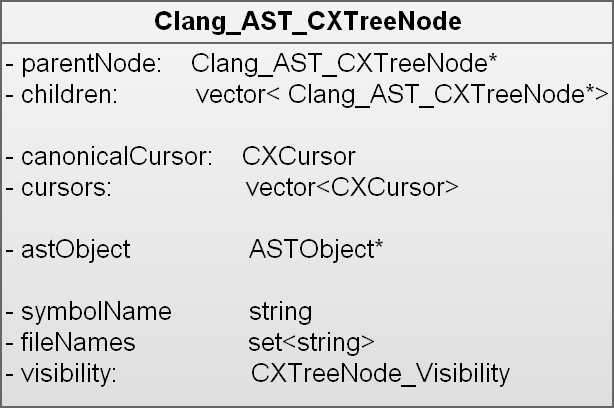
\includegraphics[scale=0.3]{Images/CXTreeNode.png}
	\caption{Members of an intermediate tree node}
	\label{fig:CXTreeNode}
\end{figure}

Every node holds a pointer to its parent and all of its children, resulting in a tree structure that can be traversed in both directions. 
The \mySCName{Clang\_AST} holds a reference to the root tree node and a map that links canonical cursors to intermediate tree nodes (for faster access).

After the translation unit has been parsed using \mySCName{clang\_parseTranslationUnit}, all the children of the translation unit cursor will be visited with the help of \mySCName{clang\_visitChildren}. Every visited child cursor is checked, whether an intermediate tree node has already been created for it - based on the child's canonical cursor. If so, the tree node is retrieved, the visited cursor added to its list of cursors and the children are visited. Visiting the children for an already existing tree node is necessary, as the the new found cursor may contain more children (for example if it is a class definition).\\
If no tree node is existing for the canonical cursor, then, depending on the cursor's kind, a new tree node is created, inserted into the tree and added to the map that links canonical cursors and tree nodes. A lot of AST nodes are not needed for language binding. Thus, the first filtering happens at this stage and tree nodes for the intermediate AST will only be created for the following C++ entities:\\global and static variables, unions, typedefs, structs, (templated) classes, (templated) functions, function parameters, member functions, constructors, destructors, fields (data members), enums, enum constants, namespaces, template parameters, template arguments and linkage specifiers (e.g. 'extern ''C''').\\
From this list, it is obvious, that the intermediate AST will only have details up to function-level. Source code inside functions is not considered. 

\subsection{User-based filtering}

Parsing code that includes heavy libraries, like the C++ standard library or Boost\todo{ref}, results in a massive AST containing classes and other entities that the end-user might not want to create language bindings for and can as such be considered noise. With the help of different user-provided filters, the amount of nodes in the AST can be vastly reduced. 

At the time of creation, every tree node has been marked as \textbf{not visible}. Only nodes that are marked \textbf{visible} or \textbf{referenced} will appear in the final simplified AST. Referenced nodes are AST nodes that were initially filtered out, but are used by other nodes as a parent or for type information. As such, these nodes are an integral part of a consistent AST, where every node is a) supposed to be reachable while traversing the tree and b) expected to exist in the final tree when being referenced by an another node.

In the filtering step every node of the intermediate tree will be checked.

First the filename is checked with the help of a user-given regular expression. As a tree node may combine multiple cursors, the filenames of all these cursors are retrieved and matched against the regular expression. If none succeeds, the node and all its children are considered \textbf{not visible}.

The second filter matches the complete symbol name of a node (mangled with all parent names added upfront) against a regular expression. Some nodes, like linkage specifiers, will not be checked, as they do not have a name. If the symbol name check fails, then - depending on the kind of node (for example namespace) - the algorithm will still check the visibility of the children as the symbol name filter may apply to those.

The third filter will check the member access of a node - whether it is private, protected, public or any combination of those. For language binding, non-public members are not needed as they can not be referenced by glue code.

If the tree node passes all three filters, it will be marked as \textbf{visible}. As explained in more detail in the next section, an \mySCName{ASTObject} - a node of the final AST - will be created and stored in the intermediate tree node. Also, all parent nodes (that are marked as \textbf{not visible}) will be marked as \textbf{referenced} and thus appear in the final AST.

Depending on the kind of node, the visibility of the children will be checked recursively.

\todo{current filtering vs future}

\subsection{The final AST}

The final simplified AST is a tree structure made of classes that inherit from
\mySCName{ASTObject}. A single class exists for every kind of AST node. Only linkage specifiers will not appear in the final AST. The descendants of \mySCName{ASTObject} hold information according to their kind. \mySCName{ASTObject\_Function}, for example, holds information about its return type and parameters. Clang treats static data members as variable declarations. The simplified AST will treat them as instances of \mySCName{ASTObject\_Field} that have the static-member set to true.\\
An overview over the existing subclasses of \mySCName{ASTObject} can be found in \myRefFigure{fig:ASTObjectUML}.

\begin{figure}[p] % h = here
	\centering
		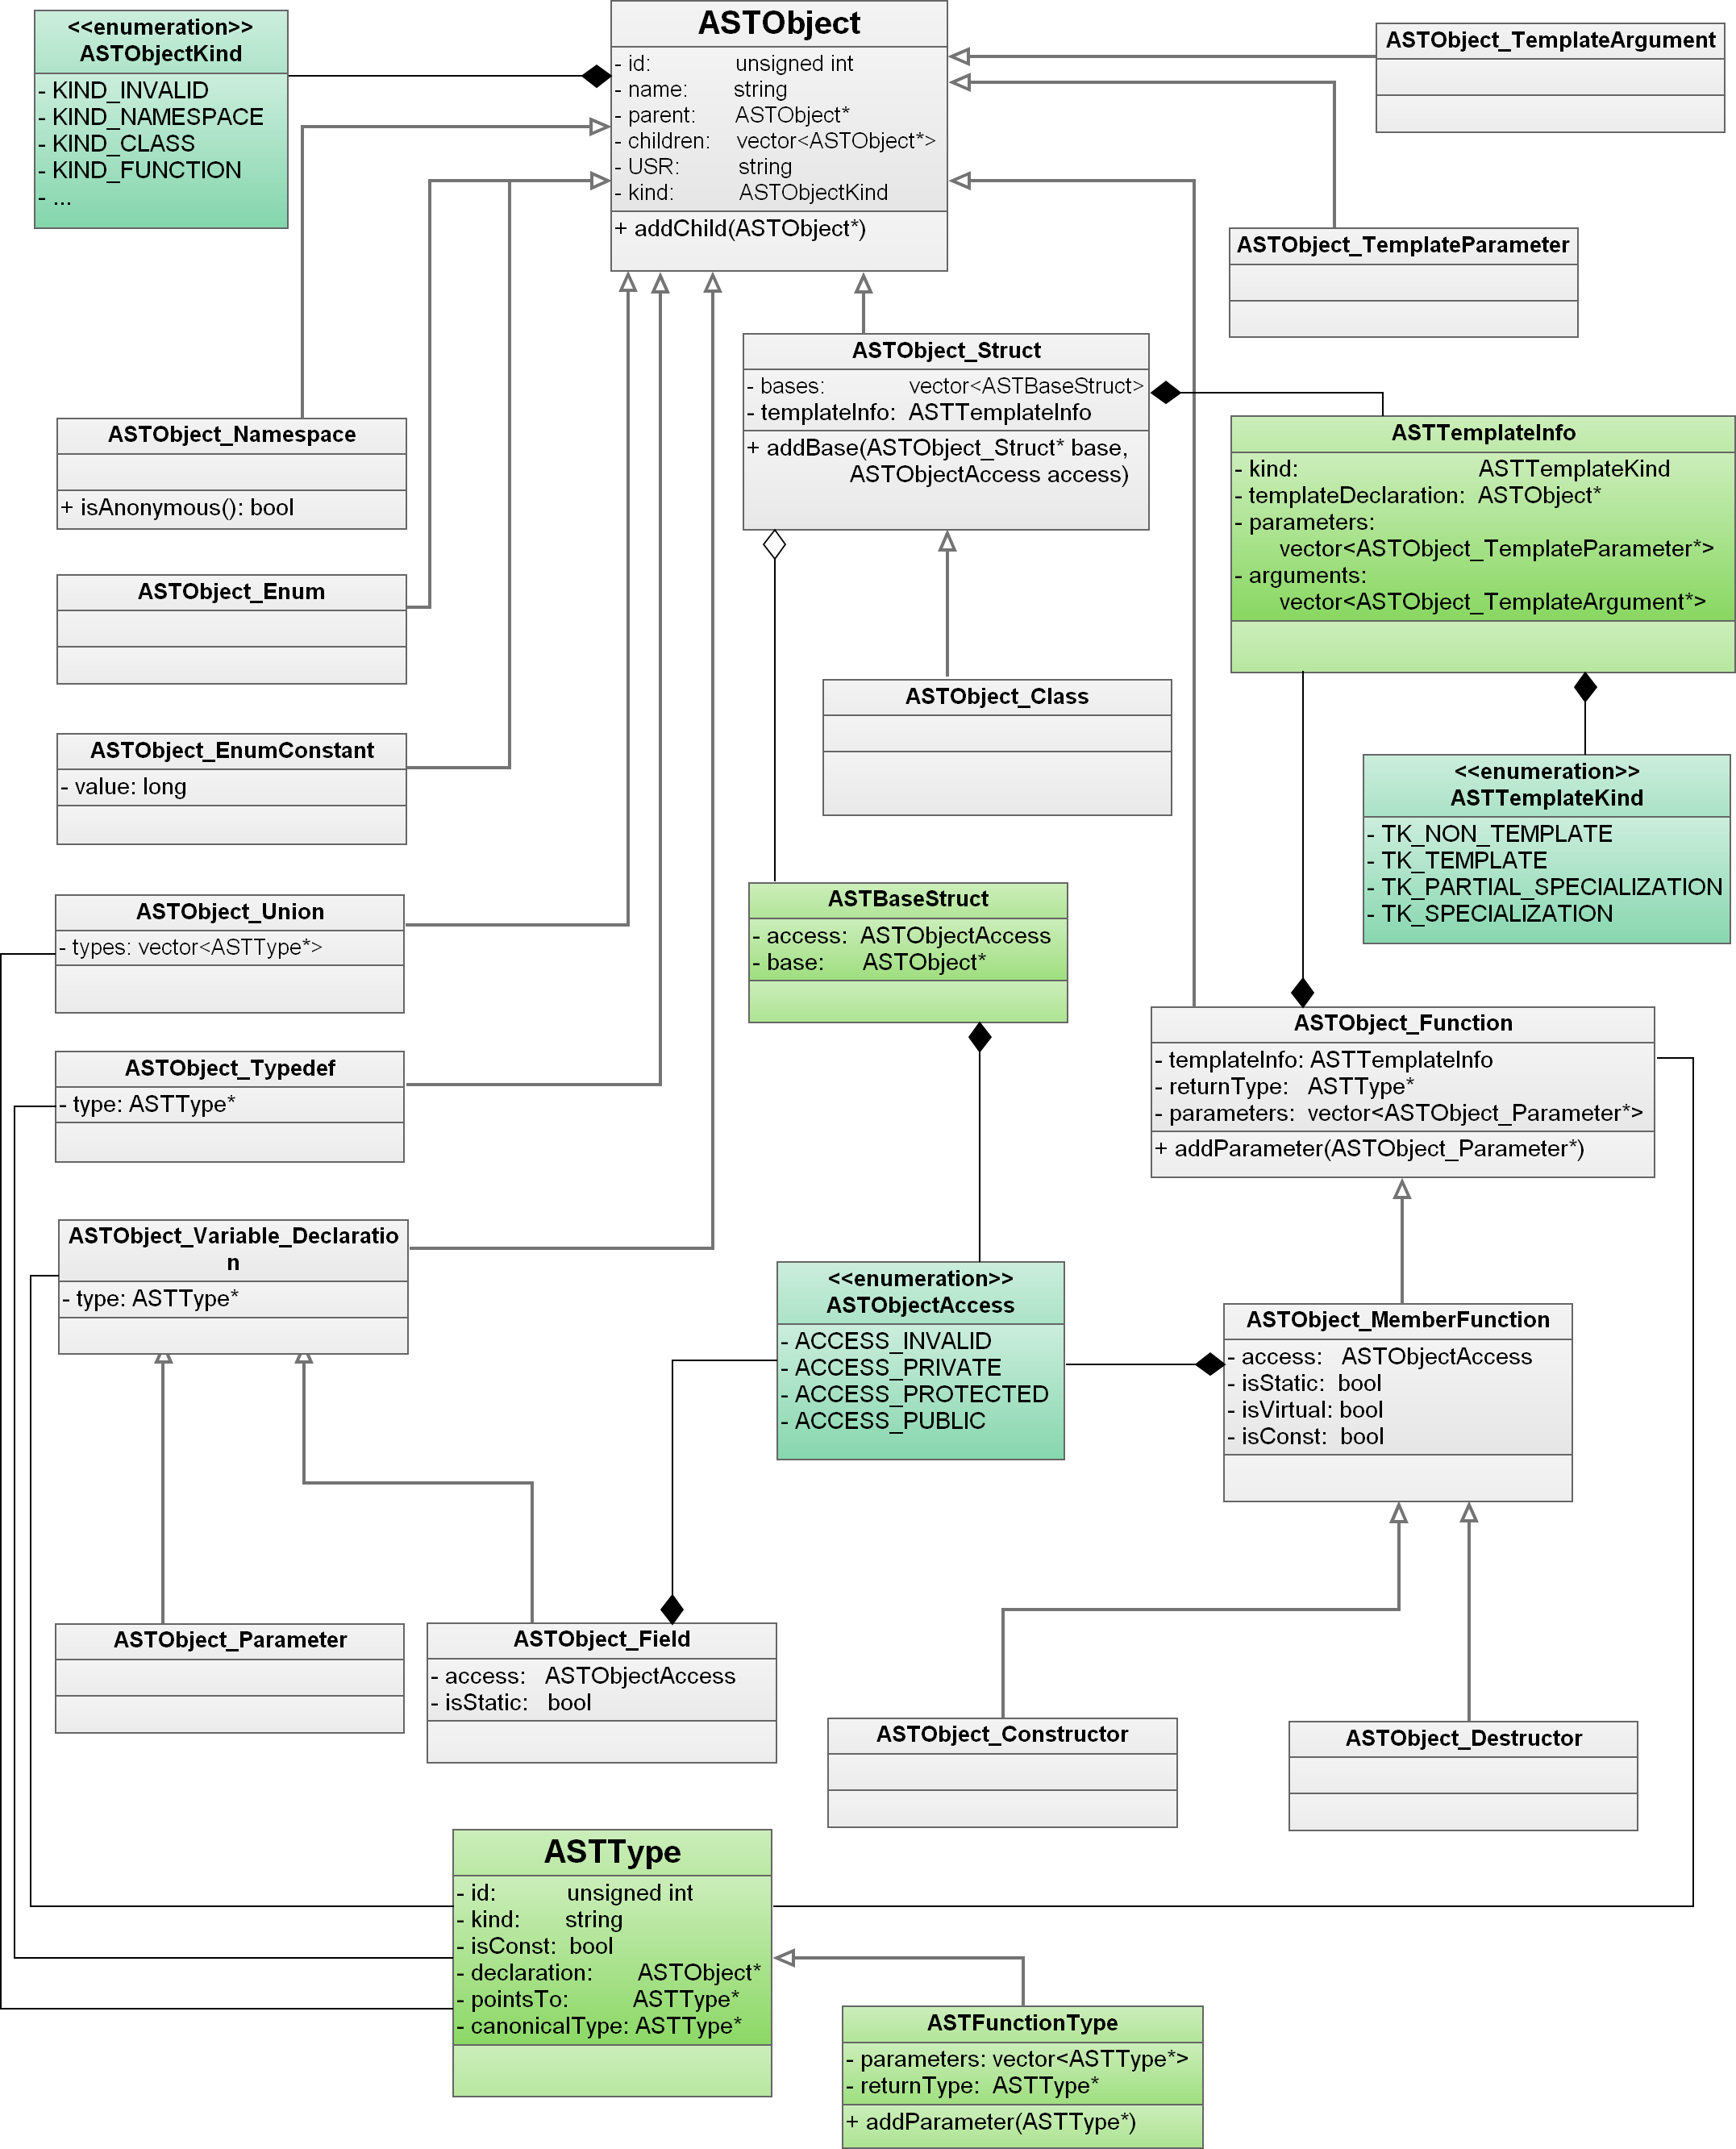
\includegraphics[scale=0.2]{Images/ASTObjectUML.png}
	\caption{ASTObject classes and ASTType (not all associations shown)}
	\label{fig:ASTObjectUML}
\end{figure}

\newpage
Just like \mySCName{Clang\_AST\_CXTreeNode}s, the \mySCName{ASTObject}s store a pointer to their parent and children and thus form a tree that can be traversed in both directions.

\mySCName{ASTObject}s are created whenever an intermediate tree node is marked \textbf{visible} or \textbf{referenced}.

When creating the specific \mySCName{ASTObject}s, the information belonging to the nodes is retrieved using the functions provided by libclang. This includes template information, base information, member access, function parameters, type information and much more.

Type information - exposed by libclang as CXType - will be saved as instances of \mySCName{ASTType}. Apart from the kind of type (int, float, pointer, reference, record, typedef, etc.), \mySCName{ASTType} also stores information about the declaration \mySCName{ASTObject} it refers to (for record and typedef types), the pointee-type (for pointer and reference types) and whether the type is declared as ''const''. It also stores a pointer to the canonical type, which is the same type in its completely desugared form (all typedefs removed). \mySCName{ASTFunctionType} stores the return type as well as the types of all parameters of a function type.

While creating \mySCName{ASTObject}s and \mySCName{ASTType}s other \mySCName{ASTObject}s and \mySCName{ASTType}s will be referenced. In case the belonging intermediate tree nodes are marked as \textbf{not visible}, these nodes and all their parent nodes have to be marked as \textbf{referenced} and their \mySCName{ASTObject}s created, so they can be referenced. In some cases, for example for implicit template specializations, the intermediate tree nodes are also not existing and have to be created and inserted before creating the according \mySCName{ASTObject}.

In the final step, the intermediate tree is traversed from top to bottom and the existing \mySCName{ASTObject}s are connected with the next existing \mySCName{ASTObject} up in the parent chain. Remember: for some nodes, like linkage specifiers, no \mySCName{ASTObject}s have been created.

The final simplified AST is now finished and ready for further use in the application. From this point on, libclang is not used any more.

There are AST nodes and types that are not exposed by libclang. If such a node or type is detected, a warning message is stored in a logger that belongs to the \mySCName{Clang\_AST}.

\newpage
\subsection{From source code to simplified AST}
\SingleSpacing
\begin{lstlisting}[language=C++, caption=Example input code for CPPAnalyzer]
namespace SomeNamespace
{
	class SomeClass;
	
	class SomeClass
	{
		int member;
	};
	
	int aFunction(float param)
	{
		float res = param * 3;
		return res;
	}
}

extern "C"
{
	void dontFilter(SomeClass pInstance){};
}
\end{lstlisting}
\OnehalfSpacing

\vspace{15pt}
\begin{figure}[h] % h = here
	\centering
		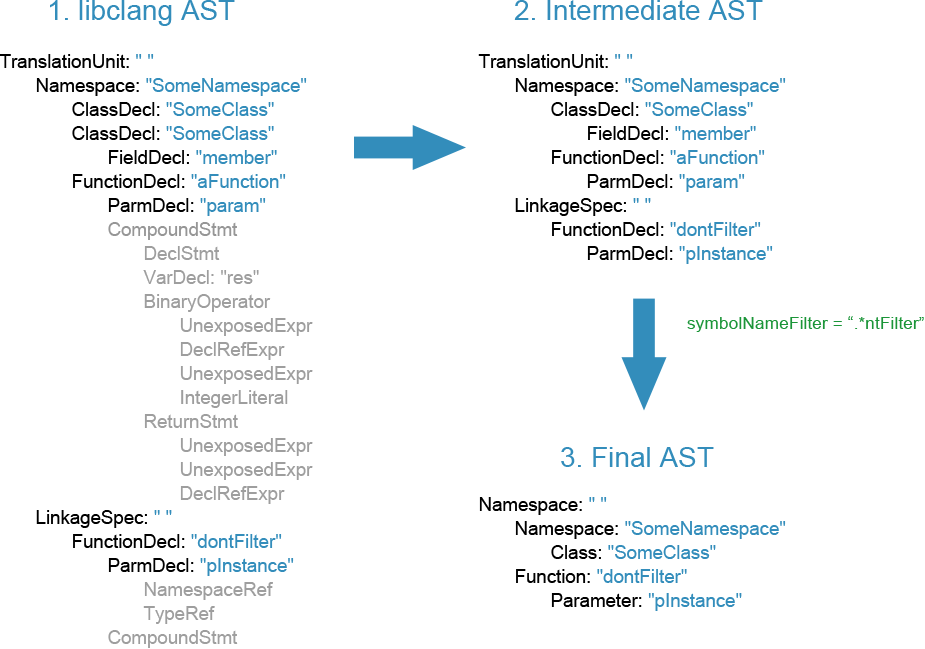
\includegraphics[scale=0.45]{Images/TreeExample.png}
	\caption{Comparison of generated ASTs}
	\label{fig:TreeExample}
\end{figure}


As can be seen in \myRefFigure{fig:TreeExample}, the AST clang produces contains a lot of unnecessary information. The intermediate AST removes many kinds of cursors and combines multiple declarations for the same entity. The final AST filters based on user-given options. In the example the function \mySCName{dontFilter} is the only node that was marked \textbf{visible}, because it is the only node that matched the symbol name filter. \mySCName{pInstance} is referenced as a parameter of \mySCName{dontFilter}. \mySCName{SomeClass} is referenced by the \mySCName{ASTType} used in \mySCName{pInstance}. Thus \mySCName{SomeClass} and its parent \mySCName{SomeNamespace} are marked as \textbf{referenced} and as such are visible in the final tree. Note that the children of \mySCName{SomeClass} are not visible.

\section{Exporting AST to JSON}

\section{libclang and the C++ standard library}
